% Author : Pierre-Henri Horrein
% Copyright : Telecom Bretagne, 2013

% Définition du document
\documentclass[t,10pt,pdftex]{beamer}
\usetheme{tb}
\usepackage{ucs}
\usepackage[utf8x]{inputenc}
\usepackage{textcomp}
\usepackage{graphicx}
\usepackage[french]{babel}
%\setbeamertemplate{navigation symbols}[horizontal]
\usepackage{multicol}
\graphicspath{{figs/}}

%\vspace{-1.5in}
% Entre [], le titre raccourci pour le bas de page, 
% Entre {}, le titre complet pour la page de garde
\title[Adversarial Attacks]{Adversarial Attacks }

% Nom de l'auteur
\author{Requirement Specification Document}
% Date de la présentation (bas de page)
\date{02/11/2018}

\linespread{1.5}

\begin{document}



\inserttitlepage

\begin{frame}[c]
\frametitle{}
\vspace{0.5in}
This \textbf{Requirement Specification Document} has been prepared by Jessal V. A., Adhithya S., Janaki Keerthi and Jayasoorya Jithendra under the guidance of \textbf{Prof. Rajasree R.}, Assistant Professor,\\College of Engineering Trivandrum.
\end{frame}


\begin{frame}[c]
	\frametitle{Contents}
	
	\tableofcontents[hideallsubsections]
	
\end{frame}

%\AtBeginSubsection[] {
\AtBeginSection[] {
 \begin{frame}[c]
 \frametitle{}
   \small \tableofcontents[hideallsubsections,sectionstyle=show/shaded,subsectionstyle=hide/hide/hide ]
\end{frame}
}

\section{ Introduction}
\begin{frame}
	\frametitle{Introduction}
	\begin{itemize}
		\item Adversarial attacks on images refers to applying small\\perturbations on them so that they are misclassified by\\the neural network
		\item The model predicts an incorrect answer with high confidence
		\item But the attack can be constructively used in image captchas
		\item The aim of the project is to prevent image captchas and\\social media pictures from being correctly classified by bots
	\end{itemize}
\end{frame}

%\section{Security Threats}
\begin{frame}
	\frametitle{Security Threats}
	\begin{itemize}
		\item Imagine replacing a stop sign with an adversarial example of it.\\
		That is, a sign that a human would recognize instantly but a\\neural network would not even register.
		\item Biometric security systems would also be at risk and illegal or improper content could potentially bypass neural-network-based content filters by using adversarial examples.
	\end{itemize}
\end{frame}
\section{Problem definition}
\begin{frame}
	\frametitle{Problem definition}
	\begin{itemize}
		\item To perform adversarial attacks on Image captchas to prevent\\bots from automating captcha tests.
        \item To perform adversarial attacks on Personal Social Media\\pictures to prevent models from detecting face.
        
	\end{itemize}
\end{frame}
\section{Design}

\begin{frame}
	\frametitle{}
%	\begin{flushleft}
	\begin{figure}
	    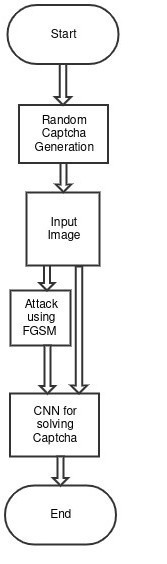
\includegraphics[width=1.25in,height=3.25in]{uml.jpg}
	\end{figure}
%	\end{flushleft}
\end{frame}


\section{Fast Gradient Sign Method}

\begin{frame}
	\frametitle{Fast Gradient Sign Method}
	 FGSM computes an adversarial image by adding a pixel-wide perturbation of magnitude in the direction of the gradient. This perturbation is computed with a single step, thus is very efficient in terms of computation time.\\\bigskip
        
        \centerline{$X^{adv} = x + \epsilon . sign(\nabla_{x}J(x, y_{true}))$}\\
       \begin{flushleft}
        where X is the clean input, $X^{adv}$ is the perturbed adversarial example,\\J  is the classifier's loss function,   $y_{true}$  is the true label for the input x.\\
        \end{flushleft}
\end{frame}

\begin{frame}
\frametitle{Attacks on Images}
%\begin{flushleft}
\hspace{-0.5in}
		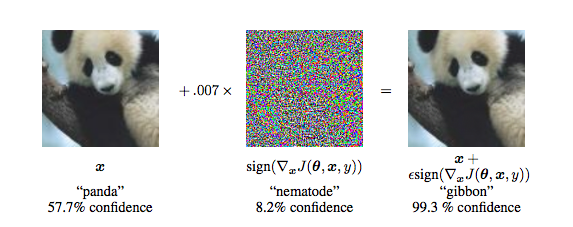
\includegraphics[width=3.25in]{goodfellow.png}
%\end{flushleft}\\
\hspace{4.5in}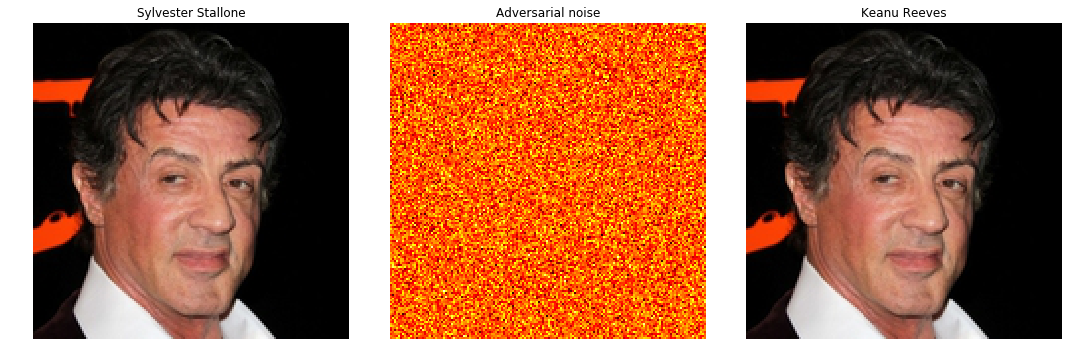
\includegraphics[width=3in]{social.png}

		\end{frame}
		
\section{Performing the Attack}
\begin{frame}
\frametitle{Performing the Attack}
\begin{itemize}
    \item MNIST dataset of 70,000 images is used for the pu
\end{itemize}
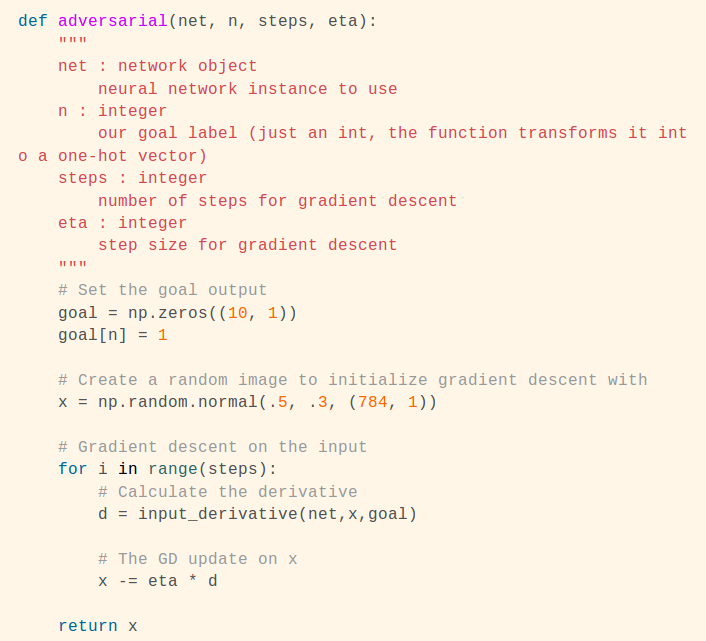
\includegraphics[width=3.25in,height=2.5in]{code.png}

\end{frame}



\section{References}
\begin{frame}
\frametitle{References}
\footnotesize{
\begin{thebibliography}{99}

\bibitem[Ian J. Goodfellow, Jonathon Shlens & Christian Szegedy, 2015]{p1}Ian J. Goodfellow, Jonathon Shlens & Christian Szegedy (2015)
\newblock \emph{"Explaining And Harnessing Adversarial Examples"}

\bibitem[Gamaleldin F. Elsayed, Ian Goodfellow, Jascha Sohl-Dickstein , 2018]{p1}Gamaleldin F. Elsayed, Ian Goodfellow, Jascha Sohl-Dickstein  (2018)
\newblock \emph{"Adversarial Reprogramming of Neural Networks"}

\bibitem[F. Tramèr et al. , 2017]{p1} F. Tramèr et al. (2017)
\newblock \emph{“Ensemble Adversarial Training: Attacks and
Defenses” }

\bibitem[Hassan Gomaa, 2011]{p1}Hassan Gomaa (2011)
\newblock \emph{"Software Modelling And Design-UML, Use Cases, Patterns, and
Software Architectures"}
\end{thebibliography}
}


\end{frame}


%------------------------------------------------




\end{document}
